\documentclass[11pt]{revtex4}

\usepackage{graphicx}
\setlength\textwidth{6.25in}
\setlength\topmargin{-0.25in}

\begin{document}

\title{Final report: Adaptive Hybrid Simulations of Solvated Reactions}

\author{Noam Bernstein}
\affiliation{Center for Computational Materials Science, Naval Research Lab Code 6390, 4555 Overlook Ave SW, Washington DC, 20375}

\author{G\'abor Cs\'anyi}
\affiliation{Computational Mechanics Group, Engineering Laboratory, University of Cambridge, Trumpington Street, Cambridge CB2 1PZ, UK}

\maketitle

\section{Introduction}

Many chemical processes of scientific and technological importance
involve the breaking and formation of covalent bonds between atoms,
in the presence of large structures and large numbers of solvent
molecules.  Describing the bond breaking process requires a reliable
quantum-mechanical description of interatomic bonding.  However,
methods that can do this are limited to a few hundred atoms at most, but often
the reaction region is affected, directly or indirectly, by many
more atoms or molecules.  The large number of atoms required can
be described with classical interatomic potentials, but these cannot describe the bond breaking itself.  To include both of these
effects, methods that couple the different computational approaches
have been developed.  These methods are referred to as hybrid or
concurrent coupling schemes in the solid state
literature~\cite{curtin_model_simul_mater_sci_eng_2003a,csanyi_j_phys_condens_mater_2005a,bernstein_rep_prog_phys_2009a} and
as QM/MM (quantum mechanics/molecular mechanics) in the chemistry
literature~\cite{senn_topics_cur_chem_2007a,lin_theor_chem_acc_2005a}.

A number of challenges can arise in the development of a hyrid
simulation method: boundary effects at the edge of each simulation
(QM or MM) region, coupling the two regions mechanically and
electostatically, and moving the QM region (or moving atoms into
or out of a fixed region).  Various subsets of these problems have
been handled in different ways in published implementations, as we
discuss in more detail in the next section.  It is important to
determine what consitutes ``success'' for a hybrid method.  We focus
on reproducing observables (i.e. ensemble averages) in the QM region
in agreement with a full QM simulation.  Agreement with experiment
is also important, of course, but a hybrid method that agrees with
experiment when the underlying, nominally accurate, QM method does
not is probably just benefitting from a cancellation of errors, and
is unlikely to be transferable or reliable.  This statement is not
absolute: interatomic potentials could be fit to reproduce interactions,
for example dispersion forces, that are not well described by QM
method such as density functional theory (DFT).

In this project we have implemented a hybrid method based on atomic
forces that attempts to address all of these issues.  We have tested
it on a relatively challenging system, liquid water and ions solvated
in water, and shown that the hybrid method is good at reproducing
the fully QM simulation.

\section{Background}

The QM/MM approach in chemistry was first introduced by
Warshel~\cite{warshel_j_mol_biol_1976a} for the study of a reaction
in the active site of an enzymatic protein.  It has since been
applied to many systems, some recently reviewed in
Refs.\onlinecite{senn_topics_cur_chem_2007a} and
\onlinecite{lin_theor_chem_acc_2005a}.  The vast majority of QM/MM
implementations in the chemistry community begin by defining a total
energy for the coupled system.  In addition, a fixed set of atoms
or molecules is assumed to form the QM region.  While these assumptions
make it possible to construct a simulation that conserves total
energy, they lead to some limitations.  The first is that great
care is needed to terminate the QM and MM calculations that are to
be coupled together into an (ideally) seamless single system.  An
example of the sophistication needed for such coupling is described
in Ref.~\onlinecite{laio_j_chem_phys_2002a} for a molecular system, and in
Ref.~\onlinecite{sokol_int_j_quant_chem_2004a,sherwood_j_mol_struct_theochem_2003a} for an ionic solid-state
system.  The second is that it is impossible to change the contents
of the QM region, because doing so will necessarily change the total
energy.  In fact the observables that researchers are typically
interested in are actually constant temperature, not constant energy,
ensemble averages, since that is how experiments are usually carried
out.

\subsection{Methods}

\subsubsection{Variable QM region}

Some attempts to go beyond these limitations and to simulate liquids,
where diffusion is significant, have been published.  The first of
these is the ONIOM-XS method by Kerdcharoen and
Morokuma~\cite{kerdcharoen_chem_phys_lett_2002a}.  This approach is
based on the ONIOM method, which is one of the simplest approaches
for coupling different computational methods.  In ONIOM~\cite{svensson_j_phys_chem_1996a},
the total energy
$$ E = E_1(1+2) + E_2(1) - E_1(1), $$
where $E_1$ is the energy evaluated with the fast method (MM), $E_2$ is
the method evaluated with the slow method (QM), and the arguments
indicate the two regions where the two methods are to be used.  If
any covalent bonds are broken at the interface, the two calculations
on region 1 (last 2 terms in the equation) are done on passivated
clusters, where typically H atoms are used to saturate the dangling
bonds left by the missing region 2 atoms.  In ONIOM-XS, a transition
region between the two regions is defined.  When there are atoms
in the transition region, the total energy is a linear combination
of two ONIOM total energies, one with the transition region atoms
included in region 1, the other with the atoms included in region
2.  As Truhlar noted, this approach is not consistent when there
is more than 1 molecule in the transition
region~\cite{heyden_j_phys_chem_b_2007a}.  ONIOM-XS has been used
in a few applications to the solvation of
ions~\cite{kerdcharoen_j_chem_phys_2003a,hofer_j_amer_chem_soc_2005a}.

Heyden {\it et al.} developed the Adaptive Partitioning method,
which essentially solves the consistency issues of ONIOM-XS at the
expense of increased computational cost~\cite{heyden_j_phys_chem_b_2007a}.
In this method, instead of a linear combination of two calculations,
many simply-partitioned calculations are combined.  The most expensive
variant uses a linear combination of every permutation of possible
assignment of molecules in the transition region to the QM and MM
regions.  A simplified ``sorted'' variant orders the molecules in
increasing distance from the QM region, and combines calculations
that include in the QM region the nearest molecule, two nearest
molecules, three nearest molecules, and so on.  In the paper the
methods are tested on two small systems, the solvation in water of
a Li$^+$ ion, and liquid Ar.  The MM water molecules were described
with the CF2-BJH potential, and the QM region with density functional
theory (DFT) with the PBE0 density functional.  In comparison to
ONIOM-XS and Rode's Hot-Spot method, described below, the method
shows smoother forces as molecules move between the two regions,
but there is no comparison to full QM simulations.  The Ar liquid
was used to test constant energy and constant temperature calculations,
using two different interatomic potentials (Lennard-Jones and Morse),
rather than a QM and an MM description.

Hodak {\it et al.} developed a coupling scheme for two different
QM methods, Kohn-Sham DFT (KS-DFT) with a plane-wave basis~\cite{kohn_phys_rev_1965a}
and orbital-free DFT (OF-DFT) using fixed Gaussian charge
distributions~\cite{hodak_j_chem_phys_2008a}.  The mismatch between
these two methods is much smaller than between typical QM and MM
methods, so the edge effect and discontinuity problems are inherently
smaller.  The molecules change identity abruptly as the move between
the KS-DFT and OF-DFT regions.  The method is applied to liquid
water and to a protein-metal binding interaction.  The authors use
constraints to fix the geoemtry of the water molecules in the OF-DFT
region, and take care to apply a thermostat to molecules that have
changed identity to compensate for the addition or removal of
distortion potential energy and vibrational kinetic energy.  Tests
of the method for water are restricted to the dipole of a KS-DFT
water, and internal consistency (e.g. energy conservation), both
of which show acceptable results.

[NB: enough comment now on lack of description of actual coupling procedure?]

The main exception to the energy based coupling commonly used in
the chemistry community is the Hot-Spot method, first presented by
Kerdcharoen {\it et al.}~\cite{kerdcharoen_chem_phys_1996a}.  In
this approach, the system is divided into a QM region and an MM
region, with a thin transition region between them, typically a
0.2~{\AA} spherical shell around a spherical QM region.  Each
calculation is carried out separately, with transition region atoms
in both calculations, and the {\em forces} on each atom are combined
to give a complete set of forces for the simulation.   For atoms
in the QM and MM regions, the forces from the relevant calculation are used.
For atoms in the transition region, a linear combination of the two
forces $f^{QM}$ and $f^{MM}$ is used
$$f_i = x_i f_i^{QM} + (1-x_i) f_i^{MM},$$
with the cofficients $x_i$ changing smoothly from 1 to 0
as the positions vary from inner to outer boundaries of the transition
region.  Note that because these forces are not the gradients of a scalar
function (the potential energy), they do not lead to trajectories that
obey conservation of momentum or energy.  One essential part of the method
that is not explained is how the two calculations are actually coupled,
either mechanically or electrostatically.  In
nearly 80 subsequent publications by Rode {\it et al.}, this method
has been used for studying a large number ions solvated in water
and other solvents such as ammonia, as well as pure water.  Most
of these focused on metal ions and complexes, although a few
considered the hydration of other ions such as F$^-$ and
Cl$^-$~\cite{tongraar_phys_chem_chem_phys_2003a,tongraar_chem_phys_lett_2005a},
NO$_3^-$~\cite{tongraar_j_phys_chem_a_2006a},
HCOO$^-$~\cite{payaka_j_phys_chem_a_2009a}, and pure
water~\cite{xenides_j_chem_phys_2005a,xenides_j_mol_liq_2006a}.

Bulo {\it et al.} recently published two variants of the Adaptive
Partitioning method\cite{bulo_j_chem_theor_comp_2009a}, one based
on energies and the other on force mixing.  The energy mixing method
differs from Heyden {\it et al.}'s work by using different algorithms
for determining the weights of particular configurations in the
linear combination.  They also consider explicitly the effects of
the position dependent coefficients in the energy sum on the forces.
These terms are presumably also present in the original Adaptive
Partitioning method, otherwise it would not conserve energy, but
not discussed in Ref.~\cite{heyden_j_phys_chem_b_2007a}.   Bulo
{\it et al.} note that these forces can lead to fictitious barriers
for transition between the two regions.  They suggest aligning the
potential energy surfaces, but note that this cannot be done for
arbitrary configurations.  In fact, even if the potential energy
surfaces are perfectly aligned and there is no fictitious {\em
barrier}, differences in local energy {\em minima} values can lead
over time to net transport from one region to the other.  Finally,
Bulo {\it et al.} consider a force mixing method, and derive a
``bookkeeping term'' that accounts for the violation of energy
conservation.  They also state that the force mixing method, if the
energy conservation violation is small, will lead to better
trajectories than any other adaptive method.  The tests of the
method are done with two different interatomic potentials, SPC water
in TIP3P water, rather than with QM and MM.   The water radial
distribution functions with the energy mixing methods show large
artifacts, and look very different from either underlying single
model.  The force-mixing based method is much better, with minimal
disagreement.

\subsubsection{Fixed QM region}

In addition to the work in the previous subsection, a few publications
have presented results from QM/MM calculations on liquids with a
fixed set of atoms in the QM region.  To do this, the QM region was
restricted to a single molecule, or a molecule and a reacting ion;
the rest of the molecules were then effectively treated as a solvent,
which doesn't truly participate in the reaction, and can be described
with an interatomic potential.

Walewski {\it et al.} used a semi-empirical QM method, the
charge-self-consistent density-functional tight-binding (SCC-DFTB),
and the SPC model for water~\cite{walewski_chem_phys_lett_2004a}.
The coupling was energy based, with an additive expression for the
interaction between the QM and MM regions.  The method was applied
to pure water, and to the geometry and proton transfer in malonaldehyde,
a 9-atom ring molecule.  For water a single molecule was treated
with QM, and the rest with MM.  For malonaldehyde, the malonaldehyde
molecule itself was described with QM, and the solvent water molecules
with MM.  There is no comparison with full QM for pure water,
although the authors do note that the diffusion cofficients of the
two underlying models (SCC-DFTB and SPC) do not agree with each
other or with experiment.  There is no discussion of whether this
mismatch leads to artifacts, as were seen in
Ref.~\onlinecite{winfield_thesis_2009a}.

Geerke {\it et al.} used an additive, energy based coupling to
simulate H-bonding in water, and a exchange of a chloride ion from
amino chloride in a dimethyl ether (DME) solvent.  The QM region
consisted of a pair of water molecules and the reacting molecule,
respectively.  They compared various semi-empirical QM methods, and
a polarizable and non-polarizable interatomic potentials for DME,
but there was no comparison to a full QM calculation.  The authors
did find that for water, in comparison to experiment, the QM-MM
interaction terms could be fine tuned to improve the total energy
of the pure liquid more accurate, but this would make the agreement
for the water-dimer dissociation energy worse.  This is an example
of the dangers of fine tuning of such interaction parameters, and
the likelihood of reducing transferability upon such adjustment.
For the Cl$^-$ exchange reaction free energy barriers and differences
were computed from the potential of mean force (mean force on the
reacting species constrained to one point in the reaction path).

\subsection{Applications to water and anions}

In a pair of recent papers, Xenides {\it et al.} applied the Hot-Spot
method to the structure and dynamics of pure
water~\cite{xenides_j_chem_phys_2005a,xenides_j_mol_liq_2006a}.
The work focused on a comparison of 3 QM methods, Hartree-Fock (HF),
M{\o}ller-Plesset perturbation theory (MP2), the B3LYP DFT functional.
The QM regions included one molecule and a single hydration shell
(radius of 3.2~{\AA} for HF and B3LYP, 3.4~{\AA} for MP2), and also
HF with two neighbor shells (2HF, radius 5.6~{\AA}).  The interatomic
potential model was the flexible water model BJH-CF2.  The simulations
used 500 molecules, MD time steps of 0.2~fs, the Berendsen (velocity
rescaling) thermostat to keep the temperature at 298~K, and different
cutoffs for Coulombic and non-Coulombic interactions.  To analyze
the resulting structure of the water, the radial distribution
functions (RDFs) and angular distribution functions (ADFs) were
computed.  To analyze the dynamics, vibrational spectra were extracted
from velocity autocorrelation functions, and mean residence time
from tracking the identity of molecules in the 1st hydration shell.
The O-O RDFs show rather different looking 1st neighbor peaks for
the different methods, and significant 2nd neighbor peaks for all
but 2HF.  Cited experiments show a 2nd neighbor peak at room
temperature and pressure, which disappears at higher temperatures
or pressures.  The O-O coordination numbers varied from 4.2-4.9,
but no experimental comparison was quoted.  The position of the 1st
shell peak varied from 2.75-2.97~{\AA}, within the range of cited
experiments, which were described as difficult and unreliable, of
2.72-2.82~{\AA}.  The positions and coordination numbers are
summarized in Table~\ref{table:rode}.
O-O-O ADFs were fairly similar for all models,
showing a single broad peak from 50$^\circ$-175$^\circ$, with one
or two maxima around 75$^\circ$-100$^\circ$.  The dynamics showed
rather more divergence between the various QM models.  Internal
vibrational modes were all in reasonable agreement, but rotations
were not.  Rotational decorrelation times varied by factors of 10
across the different models, and no model was in overall reasonable
agreement with experiment.  B3LYP tended to lead to the longest
times, and the other models to much shorter time scales.  Mean-residence
times were also in poor agreement with experiment, with B3LYP a
factor of 2 too slow, and the other models factors of 1.5--2 too
fast compared to experiment.  The authors conclude that the average
coodination number is between 3 and 4, in agreement with experiment,
but that only 2-3 of these neighbouring molecules form H bonds with
the central molecule.  Inclusion of the 2nd hydration shell is
needed for a good description (i.e. 2HF), and electronic correlations
(MP2) have a moderate effect.  They also conclude that B3LYP provides
an overly structured water network, with too slow dynamics.  One
possible caution is that the Berendsen thermostat does not give a
canonical ensemble, and may corrupt the dynamics, especially if the
time constant, which was not reported, is short.  The authors also
do not investigate whether the system is in thermal equilibrium,
which has sometimes been a problem in systems with fast H degrees
of freedom coupled to slow degrees of freedom such as H$_2$O
rotation~\cite{winfield_thesis_2009a}.

\begin{table}
\label{table:rode}
\caption{Summary of structural parameters for pure water~\cite{xenides_j_chem_phys_2005a},
and anions~\cite{tongraar_phys_chem_chem_phys_2003a}.}
\begin{tabular}{lc|ll}
        &       & $r$ (\AA)     & Coord num. \\ \tableline
  HF    & O-O   & 2.97          & 4.9 \\
  MP2   & O-O   & 2.87          & 4.7 \\
  B3LYP & O-O   & 2.75          & 4.2 \\
  2HF   & O-O   & 2.92          & 4.2 \\
  HF    & F-O   & 2.68          & $4.6 \pm 0.2$ \\
  exper. & F-O  & 2.6--2.9      & 4--6 (4.5) \\
  HF    & F-H   & 1.74, 3.21 \\
  HF    & Cl-O  & 3.24          & $5.6 \pm 0.1$ \\
  exper. & Cl-O & 3.1--3.33     & 4--9 (6)   \\
  HF    & Cl-H  & 2.42\\
\end{tabular}
\end{table}

Tongraar {\it et al.} applied the Hot-Spot method to the
hydration of Cl$^-$ and F$^-$ using the HF method for the
ion and one to two solvation shells, and the BJH-CF2 interatomic
potential~\cite{tongraar_phys_chem_chem_phys_2003a,tongraar_chem_phys_lett_2005a}.
The authors used QM regions of 7.2--8.0~{\AA} for F$^-$, and 9.2~{\AA} for
Cl$^-$, and fit ion-water pair-potential interactions to QM calculations.
Molecular dynamics parameters were the same as in the pure water
simulations discussed above, except for the unit cell size which included
only 199 water molecules.  The structure was characterized in terms of
RDFs and ADFs, and compared to previously published interatomic potential
simulations and experiments.  Peak heights and coordination numbers are
summarized in Table~\ref{table:rode}.  These results are in reasonable
agreement with experiment, although the range of experimental results
is large.  The authors do note that for some of the coordination numbers,
for example number of water H's near an O atom, the computational results
are sensitive to the precise distance cutoff for ``nearest neighbors.''
The authors also compared RDFs and ADFs for bulk water molecules to water
molecules in the ions' 1st solvation shells, to see how the binding to
the ion changes the water molecules' internal structure.   They find that
compared to the bulk water molecules near F$^-$ have a weaker, longer OH
bond, and broader distribution of H-O-H angles.  These effects are even
stronger near the Cl$^-$ ion.  They also compure mean residence times,
and find that exchanges from the 1st hydration shell are slower for water
neighbors of F$^-$ than bulk water neighbors, but dynamics near Cl$^-$
are similar in speed to bulk water.

[NB: done?]

% Tongraar Chem Phys Lett 2005
%   (BLYP too rigid)
%   QM region 8.0 A, 9.2 A (F, Cl)
%   HF, BJH-CF2
%   199 waters, 0.2 fs
%   75K ts data
%   pure water, 4.0 A QM region
%   smooth forces over 0.2 A
%   ADFs
%     X-O-H
%     X: Ow low peak at 15, med peak at 110
%        F v. high peak at 15, med peak at 110
%        Cl med peak at 15, low peak at 110
%   various RDFs - bulk vs. Cl solvation vs. F solvation
%     O-H bond length
%       bulk: med
%       F - longer, broader
%       Cl - shorter, sharper
%     H-O-H angle
%       bulk: largest, med height peak
%       F smaller, med height peak
%       Cl - even smaller, sharper peak
%     power spectra:
%       Q1, Q2, Q3 - diffs
%     Table 1
%                 CN      time (depending on min time to count exchange)
%       bulk      4.7     0.2, 1.36
%       F         4.6     0.4, 2.46
%       Cl        5.6     0.22, 2.05
 
 
 
% Tongraar Chem Phys Lett 2005
% 
% 
% Payaka J Phys Chem A 2009
% 
%   HCOO$^-$ in water.
%   HF, B3LYP
%   complexes: B3LYP geom good, HF underconverged basis to agree with correlated methods
%   CF2-BJH flexible water
%   fit HCOO- -> H2O interaction to DFT (pair wise powers + Morse + Coulomb)
%   298 K, 0.2 fs, 199 waters
%   equil for 30K steps, 250K-450K steps
%   RDFs:
%     Ow-Ow, Ow-Hw, Hw-Hw,
%     O-Ow, O-Hw 
%   Ow-Ow - reasonable looking, no artifact, peak at 2.75 A,
%     back to 1 at 3.25 A
%   O-Ow
%     B3LYP shorter H bonds, lower coordination than HF
%   O-Hw
%     both higher coord (3.14, 2.71) than experiment (2.5),
%       but broad peaks, so sensitive to exact integration cutoff
%     BLYP gave 2.45, PW91 gave 2.12-2.66
%   O-Ow and O-Hw water # distributions
%     time dependences
%   various bond length, angle distributions
%   mean residence times
%     longer than pure water for HF
%     shorter than pure water for B3LYP
%     B3LYP pure water known to be too slow compared to exper
%   conclusion: B3LYP does bad dynamics, use HF, or better method
% 

% Tongraar Phys Chem Chem Phys 2003
%   HF, 7.6 A for F, 9.2 A for Cl (1.5 hydration shells)
%   BJH-CF2 flexible water
%   fit F/Cl -- water
%   298 K, 0.2 fs, 199 waters
%   from well equil MM, QM/MM for 20K ts equil, 40K ts sampling
%     claim 2 ps is enough
%   X-O and X-H RDFs
%   F-O: 
%     MM 2.53 A, coord 5.8 +- 0.1
%     QM/MM 2.68 A, 4.6 +- 0.2 (less well defined 1st peak)
%   F-H:
%     MM 1.56 A, 2.81 A
%     QM/MM 1.74 A, 3.21 A, broader
%   Cl-O: 
%     MM 3.15 A, 5.9 +- 1
%     QM/MM 3.24 A, 5.6 +- 1, broader peak
%   Cl-H:
%     MM 2.29 A
%     QM/MM broad, 2.42 A (to 3.2 A), not classical H bonds
%   O-F-O, O-Cl-O
%     two peaks, braod around 90, another around 150
%   various classical literature water, RDF maxima and coord @
%     F-O 2.67-3.0 A, 4.1-6.7
%       exper 2.6-2.9 A, 4-6 (4.5)
%     Cl-O 3.15-3.9 A, 5.1-8.4
%       exper 3.1-3.33 A, 4-9 (6)

% Xenides J. Chem. Phys. 2005
%   1st neigbour HF, MP2, B3LYP, also  HF w/ 2nd neighbor
%   CF2-NJH
%   RDFs
%   velocity autocorrel
%   reorientation time correl func.
%   mean residence time
% 
%   results
%     O-O RDF
%       1 shell - all very different looking 1st peaks, 
%         B3LYP much sharper 1st peak
%         second peak significant
%       2 shells - no 2nd peak. in experiment see 2nd peak
%         unless heated or pressurized
%       coordination HF 4.9, MP2 4.6, 2HF 4.2, B3LYP 4.2
%       R O-O experiments very tricky, 2.72-2.82
%     O-H RDFs
%       3 peak structure, fairly different for the various
%         methods - 2HF not great agreement with MP2
%         B3LYP better?
%     ADFs - broad, 50-175, peak around 100
%     dynamics
%       vibr, rot. freq - broad vibr spectra
%         experiment only for vibr., all agree
%       orientation time - very different, few experiments,
%         B3LYP best for 1, none good for other
%       MRT
%         B3LYP twice as slow, others factor of 1.5-2 too fast
%   conclusions
%     coord # 3-4 (??)
%     2 form H bonds to central water
%     2 neighbors needed
% 
% Xenides J Mol Liq 2006
%   HF, 2nd neigh, BJH-CF2, Berendsen thermostat (bad?)
%   500 waters,0.2 fs, cutoff Coulomb
%   rehash of prev results
%   from MRT - H-bond lifetime 0.33 ps, laser pulse spectroscopy 0.5 ps
% 


\section{Technical Approach}

We have developed a coupling method based on forces that is designed
to give accurate QM forces in the QM region.  It is most similar
to Rode's approach~\cite{kerdcharoen_chem_phys_1996a}, but with
some essential differences.  In particular, we perform the QM
calculation including not only the atoms where we need QM forces,
but also to a {\em buffer layer} of surrounding atoms.  These atoms
are present to insulate our QM region from edge effects, but their
QM forces are ignored.  We still take advantage of the methods
developed to passivate the broken covalent bonds and electrostatic
coupling when possible, but we can systematically improve the
accuracy of the forces in the QM region by increasing the thickness
of the buffer layer.  The non-buffer QM region forces are combined
with MM forces for the MM and buffer regions, as shown in
Fig.~\ref{fig:buffered_hybrid_diagram}, and used to compute
trajectories.  As noted by us and
others~\cite{heyden_j_phys_chem_b_2007a,bernstein_rep_prog_phys_2009a},
this approach does not guarantee conservation of energy or momentum.
Energy conservation is a global property of the forces as a function
of positions, because it implies that an integral of the forces
over any arbitrary closed path must be zero.  There is therefore
no known way to restore energy conservation.  Momentum conservation,
on the other hand, can be ensured for each configuration by forcing
the sum of all the forces to be zero.  We do this by subtracting
from each QM and buffer region atom an equal force that exactly
brings the overall force total to zero.

[NB: fix buffered hybrid diagram - explain big cross, fix PDF output of inkscape ]

\begin{figure}
  \centerline{\resizebox{4in}{!}{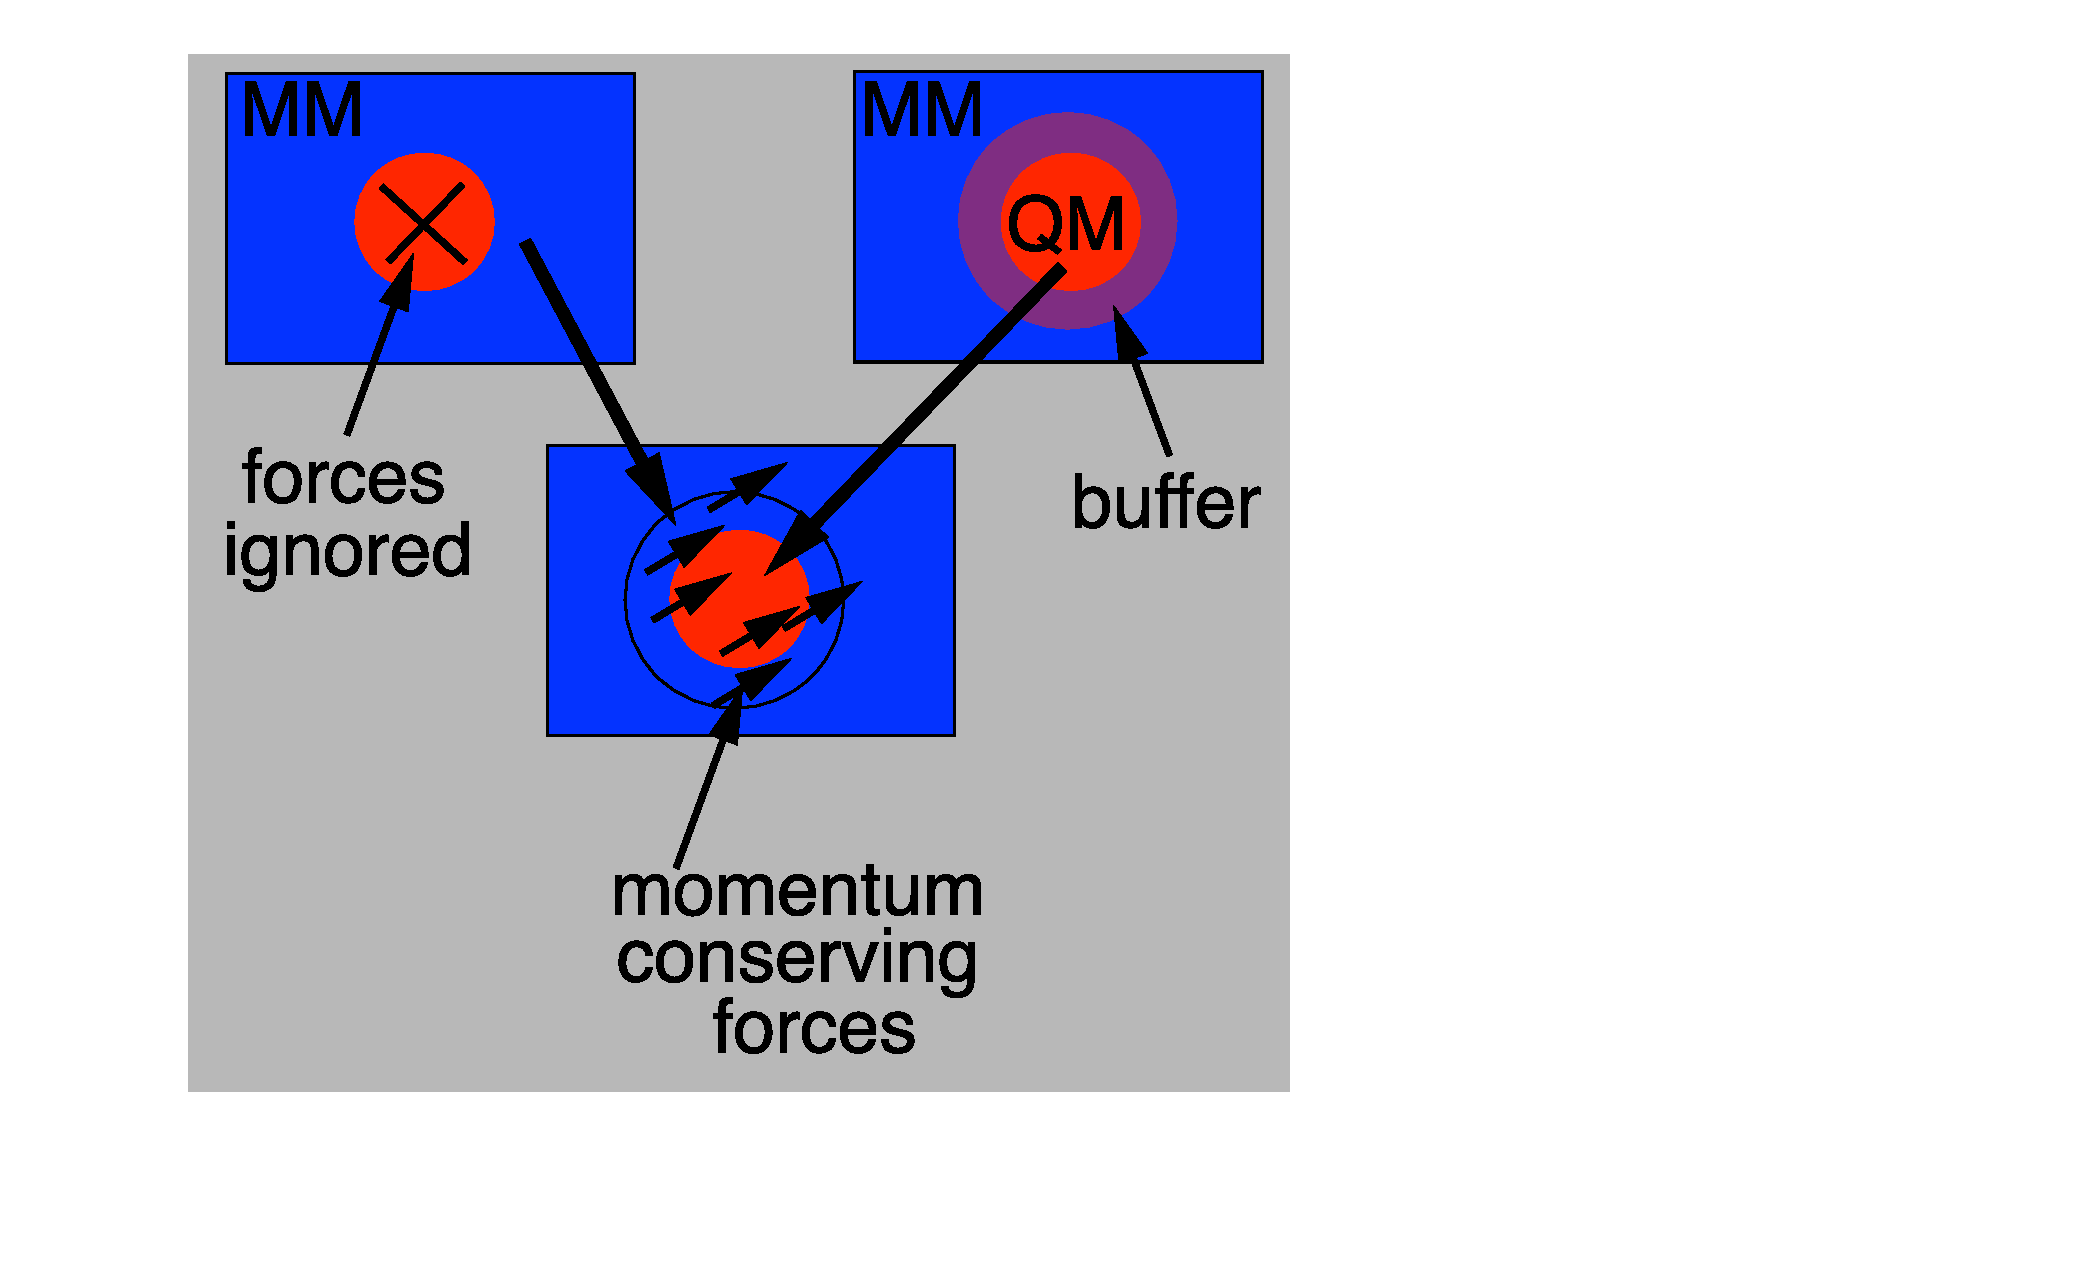
\includegraphics{buffered_hybrid_diagram}}}
  \caption{Combining of forces from MM and buffered QM calculations
           to generate a complete set of forces for trajectory calculations.
           Small arrows indicate forces applied to recover momentum
           conservation.}
  \label{fig:buffered_hybrid_diagram}
\end{figure}

The advantages of the buffered force mixing method over previously
applied methods are significant.  The forces in the QM region are
more accurate, especially in the presence of polarization as can
occur in polar regions of a protein~\cite{solt_j_phys_chem_b_2009a}.
The software has robust adaptive algorithms for QM and buffer atom
selection, tested in previous applications, enabling the transfer
of solvent molecules in and out of the QM region.  Finally, the
method has already been shown to work well for solid state systems,
where other methods used for biochemical application QM/MM are
inaccurate~\cite{bernstein_rep_prog_phys_2009a}, and will therefore
be useful for situations where a solid substrate, e.g. a solid state
support for a catalytic molecule, is present.  The underlying QM
method we use in this work is density functional theory (DFT) with
the BLYP generalized gradient approximation
(GGA)~\cite{kohn_phys_rev_1965a,becke_phys_rev_a_1988a,lee_phys_rev_b_1988a}.
For the MM region we use the CHARMM force field, which includes 2,
3, and 4 body terms (bond stretching, bending, and dihedral angle),
as well as non-bonded van der Waals type terms and fixed atomic
point charges~\cite{brooks_j_comp_chem_2009a}.  For water we use
the flexible TIP3P (3 atom-centered point charges, two bond stretch terms, one
bond bending term) parameters from within the CHARMM force field.

Both of these are implemented in the CP2K
software~\cite{vandevondele_comp_phys_comm_2005a,laino_j_chem_theor_comp_2006a,cp2k_web}.
In addition, a conventional QM/MM coupling method is also implemented
in CP2K~\cite{laio_j_chem_phys_2002a}.  When computing the MM forces,
the whole system is passed to a CP2K MM calculation.  When computing
the QM forces, a QM/MM system is passed to CP2K, treating the QM
region {\em and buffer region atoms} as QM within CP2K.  The resulting
forces outside the QM region are ignored.

The whole simulation proceeds as follows:
\begin{verbatim}
read initial configuration
repeat:
  calculate connectivity for MM force-field terms
  calculate MM forces using CP2K
  calculate QM/MM forces using CP2K
  combine MM forces in MM and buffer regions and QM/MM forces in QM region
  use combined forces to propagate configuration in time
\end{verbatim}
This method has been implemented in the {\tt libAtoms} and {\tt
QUIP} libraries, developed jointly by the PIs~\cite{libatoms_web}.
The software provides a framework that automates the connectivity
and MM force-field term calculations, invokes CP2K on a variety of
parallel computers, and carries out the time integration using the
velocity Verlet algorithm~\cite{frenkel_2002a}.  In addition, various
constraints can be applied and computable quantities tabulated.
These include structural properties, such as pair correlation
functions and neighbor numbers, temperatures, energies, and
ensemble-averaged forces that contribute the free energy difference
calculations using thermodynamic integration~\cite{frenkel_2002b}.

Past experience has shown that it is not trivial to properly thermostat
all the atomic degrees of freedom~\cite{winfield_thesis_2009a}.
This frequently overlooked issue can be manifested in various ways,
including temperature oscillations, or trajectories for light degrees
of freedom (i.e. H atoms) that do not equilibrate with the other,
heavier atoms.  We have found that a combination of Nose-Hoover and
Langevin thermostats with different parameters in the QM, boundary,
and MM regions works well to keep the system in a well-equilibrated,
constant temperature ensemble.  We use two separate Nose-Hoover
thermostats~\cite{nose_mol_phys_1984a} in the QM and buffer regions,
one for the O atoms and one for the H atoms.  The separate thermostats
ensure equilibrium between the fast and slow degrees of freedom, and
the Nose-Hoover method is most effective at handling the deviation from
energy conservation in this region~\cite{winfield_thesis_2009a}.  In the
MM region we use a Nose-Langevin thermostat, because has better ergodicity
properties than Nose-Hoover.  While it is less effective at compensating
for energy conservation deviation~\cite{winfield_thesis_2009a}, this is
not a problem in the MM region.

[NB: OK detail on thermostating now?]

\section{Results}

\subsection{Classical model}

Throughout this project, we use the TIP3P classical model for water. There are an enormous variety of classical water models in the literature. This choice is governed by two key factors. The first is that our long term goal is the simulation of biomolecules, and the classical force fields that describe them are tied to a specific water model, which is mostly TIP3P. Secondly, we are aiming to create a hybrid simulation scheme that is agnostic with respect to which two models it couples, and using a relatively crude classical water model such as TIP3P is a good way to test the ability of the coupling scheme to bridge models whose description of the system might be quite different. One modification that we introduce with respect to the original TIP3P model in the literature is to make the molecule flexible. This is helpful in the hybrid simulation context because the number of degrees of freedom does not have to change as molecules move between the QM and MM region. If we were to use a rigid water model, then when a molecule moves into the QM region, the constraints need to be released, and vibrational energy needs to be artificially put into the new degrees of freedom. Conversely, when a molecule moves into the MM region, its geometry would not be compatible with the constraints of the rigid model, and the corresponding potential and kinetic energy in these degrees of freedom need to be removed. While such a scheme is possible, and has been implemented in \cite{hodak_j_chem_phys_2008a,winfield_thesis_2009a}, we find it an unnecessary complication. To make sure that the flexible water model is still reasonable, we have computed the radial distribution function with both rigid and flexible models using two different parametrisations of the O--H bond, using two different commercial softwares, as shown in Figure~\ref{rigid-flex}. The CHARMM parametrisation is significantly better in the flexible case, and this is what we use in this project.

\begin{figure}
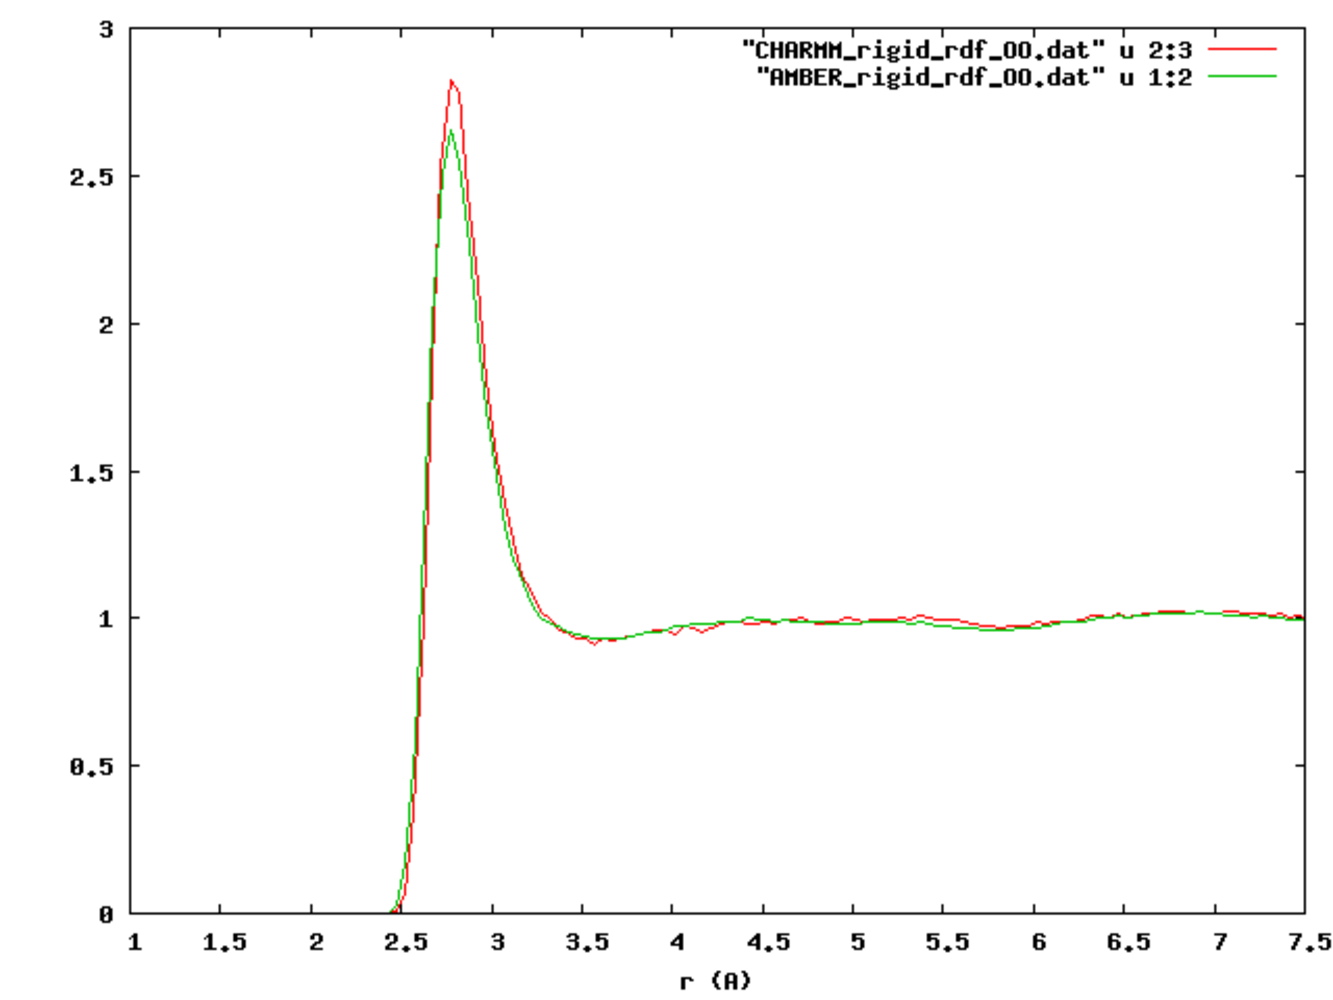
\includegraphics[height=6cm]{AMBER-CHARMM_TIP3P_rdf}
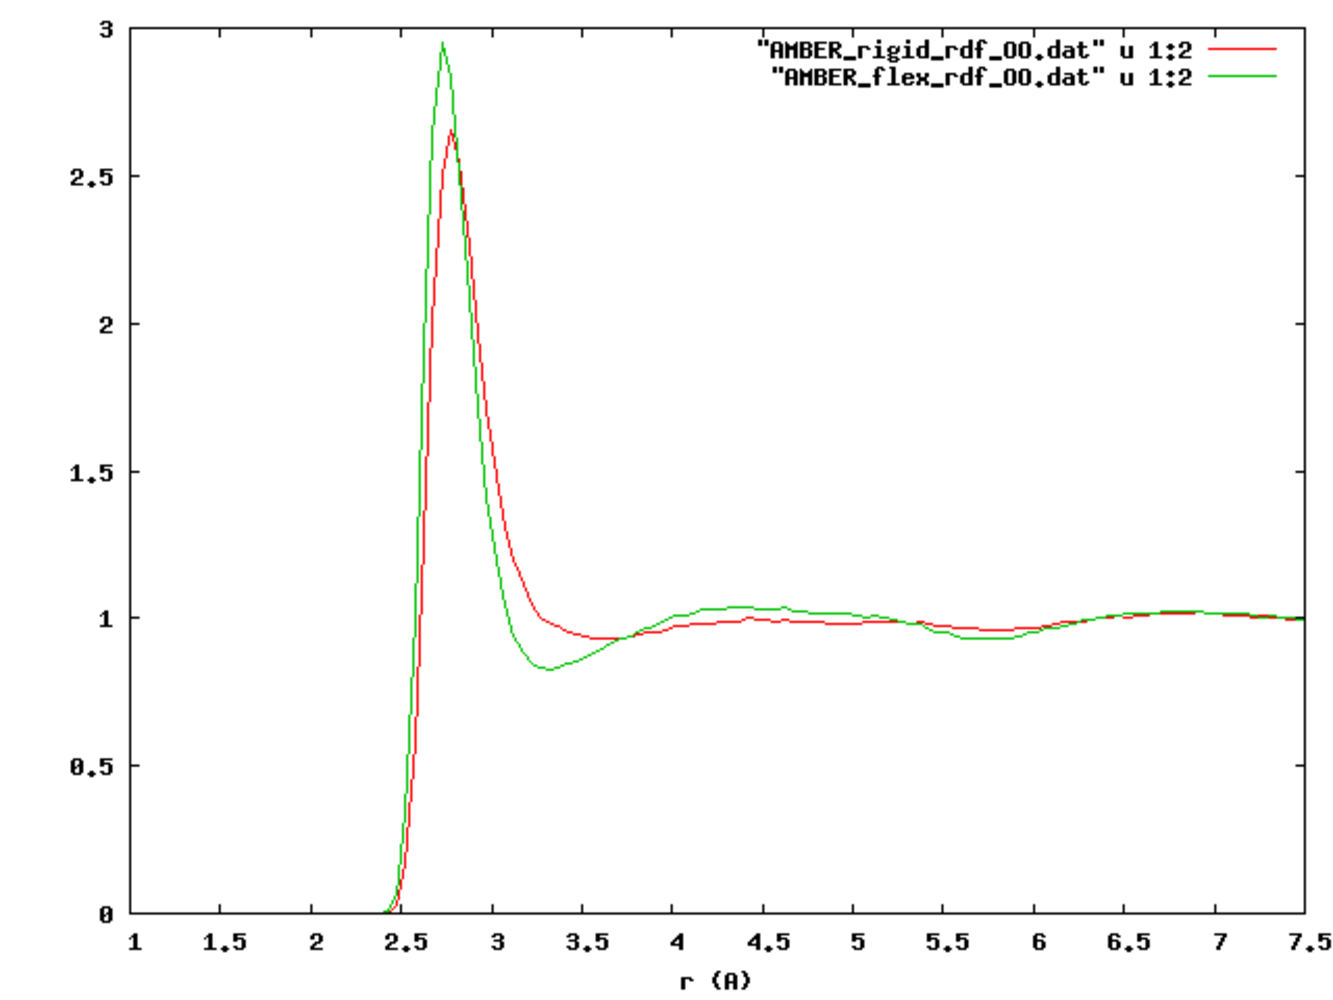
\includegraphics[height=6cm]{AMBER_rigid-flex_rdf}
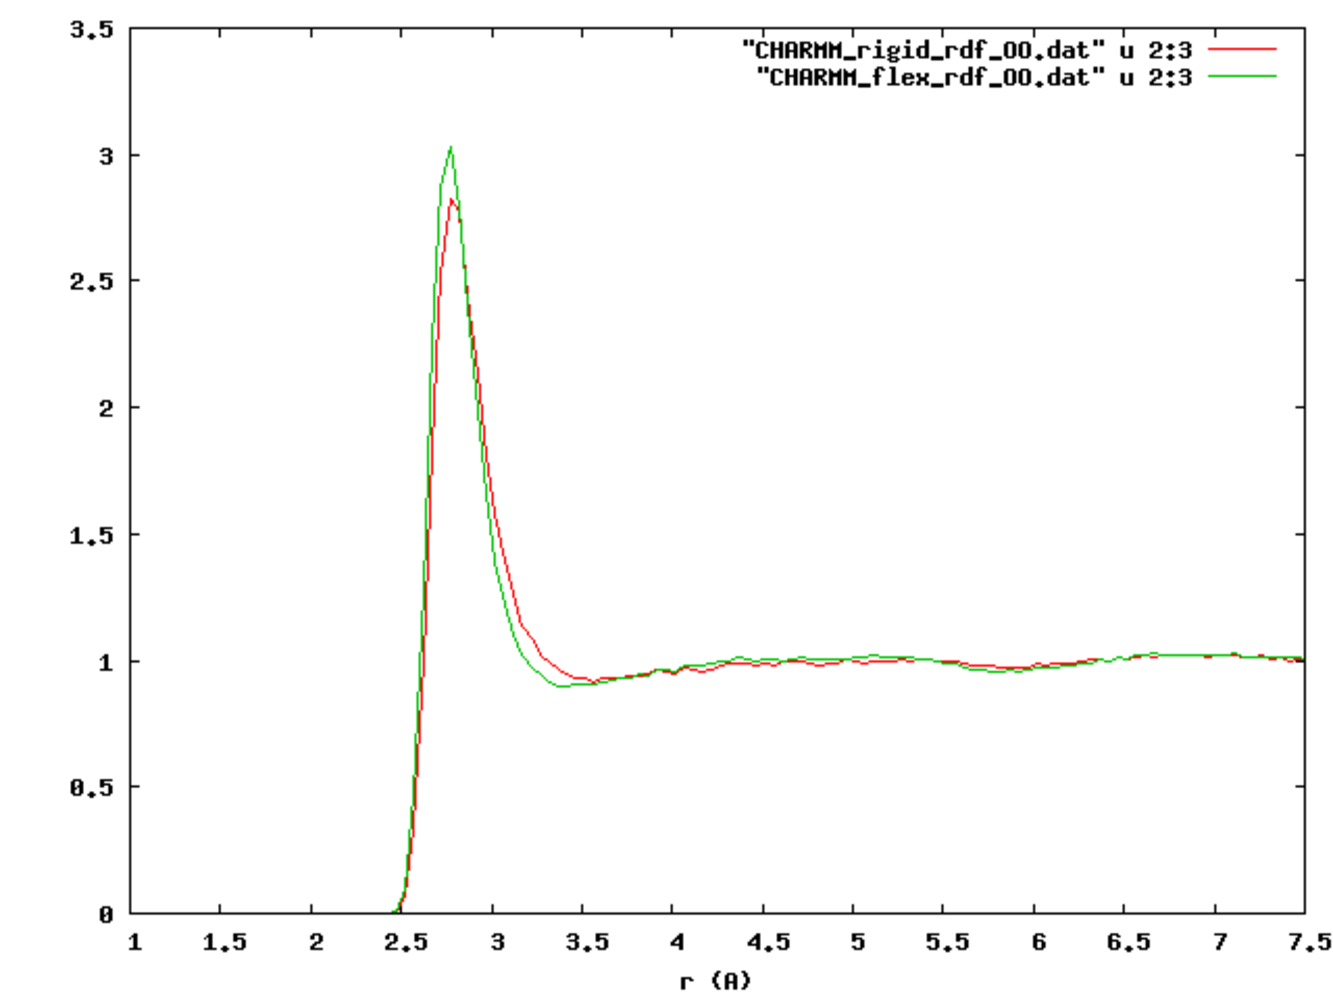
\includegraphics[height=6cm]{CHARMM_rigid-flex_rdf}
\caption{Top: AMBER and CHARMM parametrisations of the rigid TIP3P model show RDFs that match very well. Middle: the flexible TIP3P model in AMBER shows significant deviations from its rigid counterpart. Bottom: with the CHARMM parametrisation, the flexible and rigid models yield very close RDFs.}
\label{rigid-flex}
\end{figure}

\subsection{Force error vs. buffer size}

Our hybrid simulation requires an a priori determination of an appropriate buffer size in order to get forces on atoms in the QM region that are accurate enough. The minimum buffer size should be used that leads to acceptable results, because increasing the buffer size has the largest adverse effect on the cost of the simulation. Each system thus calls for some preliminary testing. Figure \ref{MCLbuftest} shows the result of such a test for a small molecule solvated in water. A buffer of about 4 to 5 \AA\ is thus reasonable. The force error is worst for highly charged atoms, as was already shown in~\cite{solt_j_phys_chem_b_2009a}.

\begin{figure}
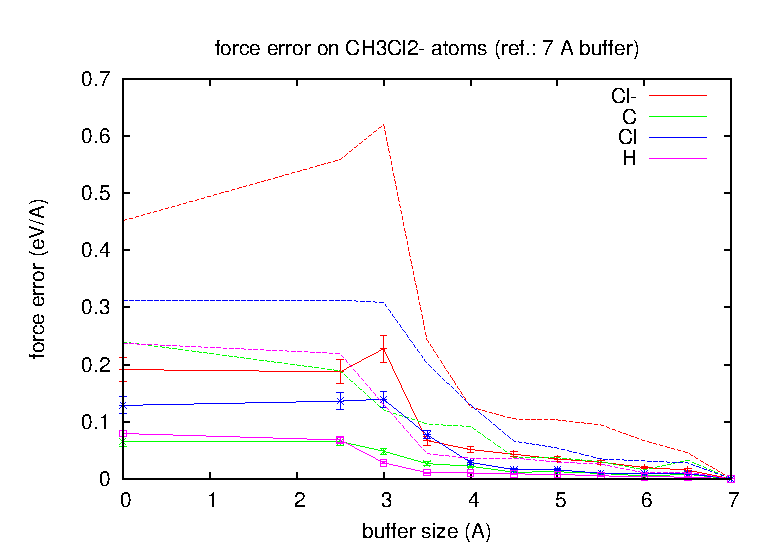
\includegraphics{force_error_MCL}
\caption{Average force component error as a function of buffer size from a BLYP/TIP3P QM/MM calculation on various atoms of methyl chloride (MCL) solvated in water. Another chloride ion is included in the simulation cell, not bonded to the molecule. The solid lines represent averages over 14 configurations, the dashed lines indicate the largest error observed. }
\label{MCLbuftest}
\end{figure}

\subsection{Chemical potential}

Even though in both our method and in the Hot Spot method only forces are used from the QM and MM models, there can be net transport between the QM and MM regions even in the case of a homogeneous liquid, which can be thought of as an effecive chemical potential difference. This net transport can arise purely due to the different diffusion constants, as illustrated in Figure~\ref{diffusion_sketch}. This is on top of any actual chemical potential difference between the models, stemming from e.g. different electrostatics. 

\begin{figure}
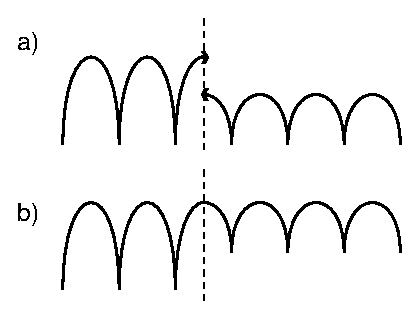
\includegraphics{diffusion}
\caption{Illustration of one way an effective chemical potential difference can arise in a force-based hybrid simulation purely from dynamical effects. In a), a series of barriers are shown between sites which are of different height for the two different models, corresponding to different diffusion constants. Even though energies are not used, the effective energy surface that a diffusion particle will feel is shown in b). The model with the higher diffusion barrier will appear to have sites with lower chemical potential. }
\label{diffusion_sketch}
\end{figure}

Such chemical potential differences can lead to unphysical density differences, in extreme cases even voids can open up in the simulation box. A practical solution is to introduce a corrective potential that compensates for the chemical potential difference. The appropriate size of the corrective potential needs to be found experimentally. Figure~\ref{density} shows the density in the simulation box for both the semiempirical PM3/TIP3P and the DFT-LDA/TIP3P hybrid simulations for different sized corrective potentials. The potentials were constant in the QM and well inside the MM regions, and had a form of a cubic spline near the transition. The width of the spline is another free parameter, and can be used to limit the adverse effect the corrective potential might have on the dynamics of the particles. A wider potential of a given depth will give rise to smaller forces. We checked that the forces arising from this potential were an order of magnitude smaller than the dynamical forces in the system, and of the same order as the forces coming from the thermostat.  Rode {\it et al.}, which used a similar approach to ours, did not comment on possible density differences.  While they did not actually show any density measurements for water\cite{xenides_j_chem_phys_2005a,xenides_j_mol_liq_2006a}, their RDFs indicate that they do not see a severe problem.  This may be because of their particular choice of QM and MM methods, the details of the QM-MM transition region, or perhaps through a cancellation of errors in their (unspecified) mechanical and electrostatic coupling scheme.


\begin{figure}
\centerline{\vbox to 5cm{\hbox to 0.5cm{a)}\vfil}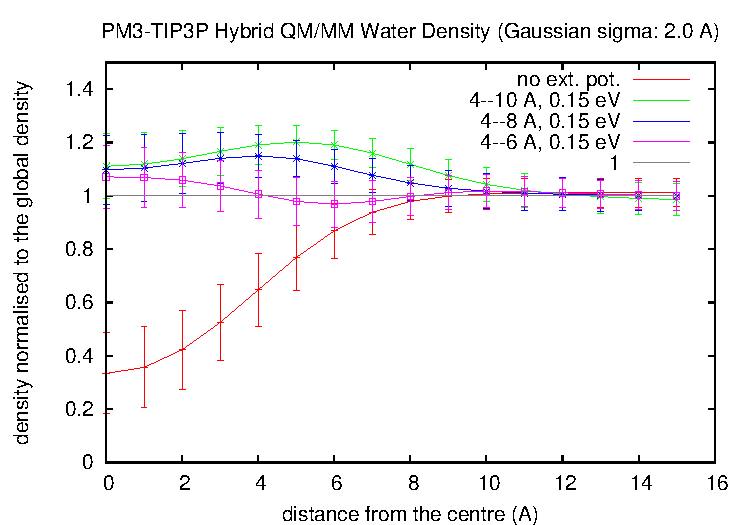
\includegraphics[width=8cm]{PM3_hybrid_4-X_0_15eV_depth_norm}
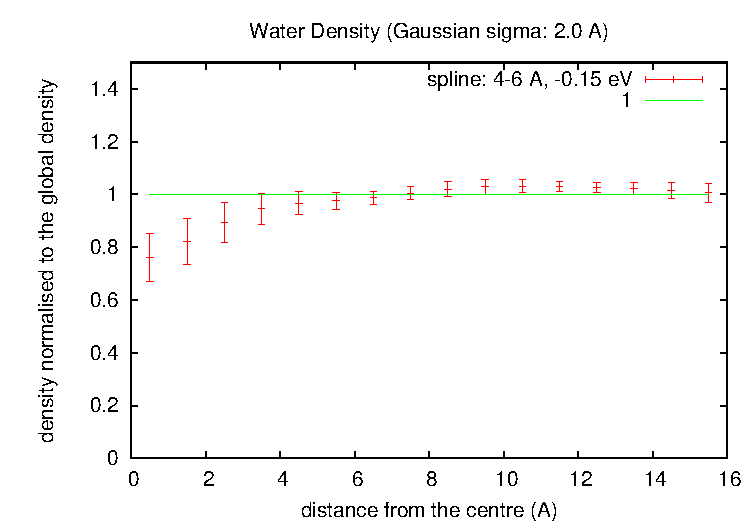
\includegraphics[width=8cm]{LDA_density_4-6_0_15eV}}
\centerline{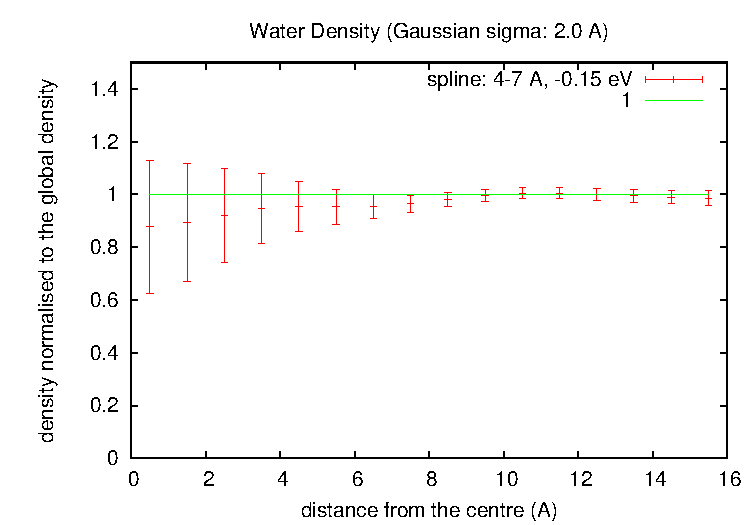
\includegraphics[width=8cm]{LDA_density_4-7_0_15eV}
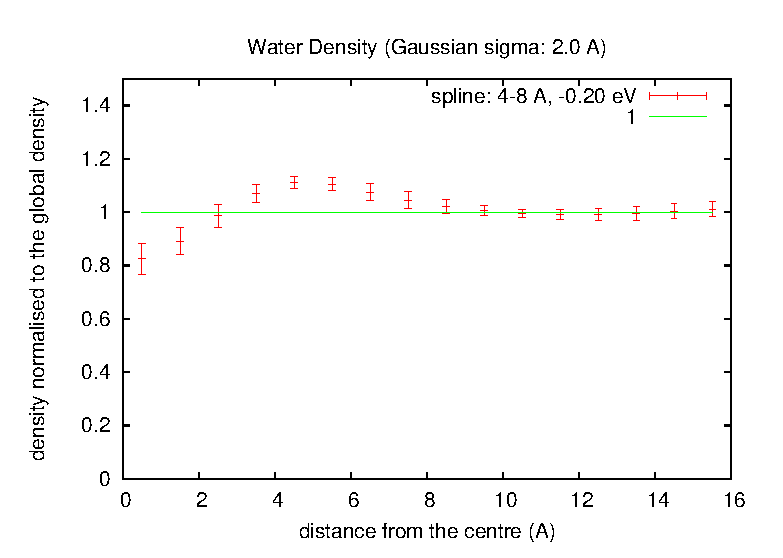
\includegraphics[width=8cm]{LDA_density_4-8_0_20eV}}
\hbox{\vbox to 5cm{\hbox to 0.5cm{b)}\vfil}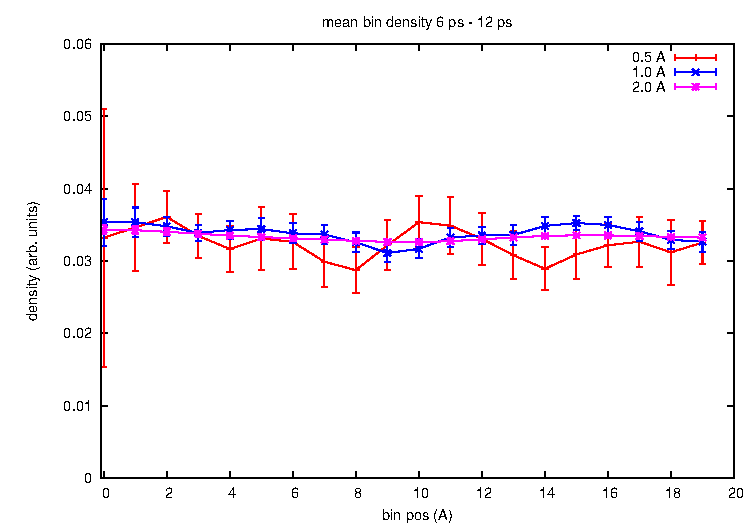
\includegraphics[width=8cm]{radial_mean_new_6_12_ps}\hfil}
\caption{a) Density of PM3/TIP3P and LDA/TIP3P QM/MM water as a function of distance form the center of the QM region for different size corrective potentials. The error bars grow towards the center of the QM zone because fewer atoms contribute to the sample there; b) water density in the BLYP/TIP3P simulation with no corrective potential. The different curves correspond to different amounts of Gaussian smoothing.}
\label{density}
\end{figure}

The parameters of the corrective potential obviously depend on which QM and MM models are used, and it turns out, rather fortuitously that for the BLYP/TIP3P combination, no corrective potential is necessary. 

\subsection{Water RDFs}
In order to compare the present method with the only practical alternative, i.e. the Hot Spot method, we calculated radial distribution functions in a hybrid simulation with and without using a buffer region.  A practical problem when considering pure water a benchmark is that DFT descriptions of bulk water are known to get the melting point wrong, and in fact at 300~K, the dynamics is very slow - in effect that system is supercooled (it does not quite freeze due to the short time scales, lack of nucleation site and small simulation cell). In order not to distract from the central issue of hybrid methodology, we carried out the tests at a somewhat higher temperature, 440~K, where the dynamics (and the radial distribution function) of DFT water better matches reality~\cite{yoo_j_chem_phys_2009a}. An added benefit of the higher temperatures is that equlibration times are shorter. Figure~\ref{water_blyp_rdf} shows the radial distribution functions for pure water and around a chloride ion using the present method and the Hot Spot method, as well as fully QM and fully MM benchmarks.

\begin{figure}
\hbox{\vbox to 8cm{\hbox to 0.5cm{a)}\vfil}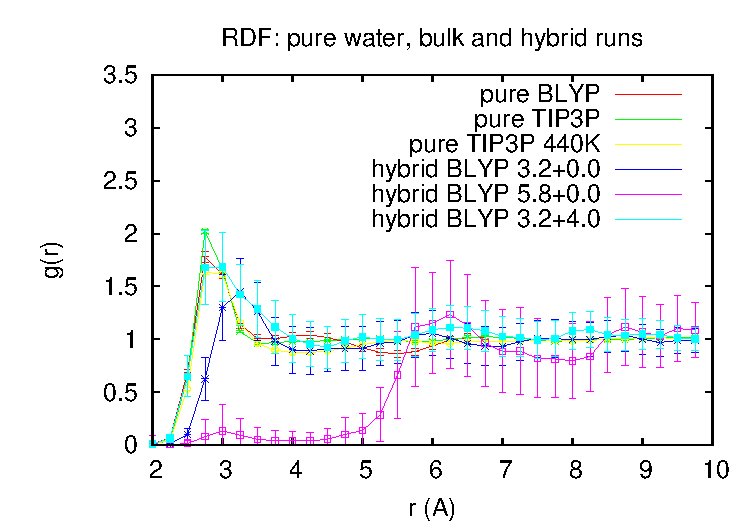
\includegraphics[height=8cm]{summary_pure_water_rdfs_G}}
\hbox{\vbox to 8cm{\hbox to 0.5cm{b)}\vfil}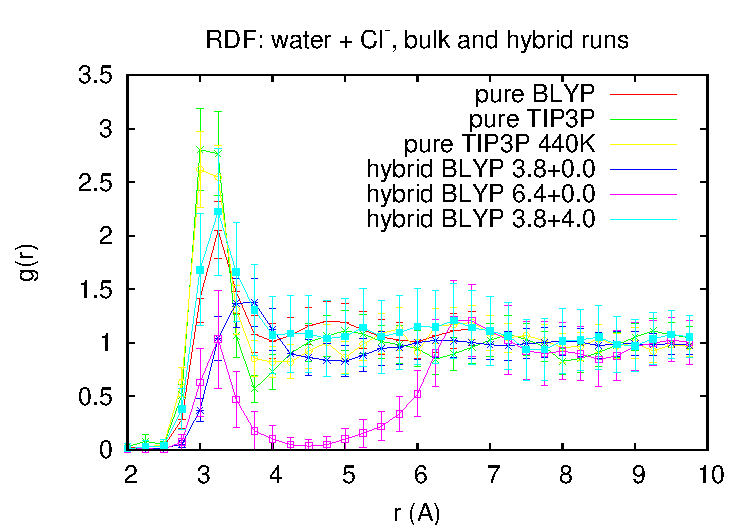
\includegraphics[height=8cm]{summary_water_Cl_rdfs_G}}
\caption{a) O--O radial distribution functions in water using the BLYP/TIP3P hybrid method, as compared with the fully BLYP and fully TIP3P models. For the hybrid curves, the first number in the label is the radius of the QM region, the second is the radius of the buffer region. Using zero buffer radius basically corresponds to the Hot Spot method; b) distribution of the Cl--O distance for a solvated chloride ion using the hybrid technique, as compared with the classical and fully quantum becnhmarks. }
\label{water_blyp_rdf}
\end{figure}
\section{Summary}

\bibliography{database}

\end{document}
